\chapter{Spacetime Symmetries}

Symmetry principles play a central role in modern theoretical physics, providing the mathematical foundation for conservation laws and the formulation of fundamental interactions. Group theory offers the natural language to describe these symmetries, both discrete and continuous. In particular, Lie groups and their corresponding algebras form the backbone of relativistic field theories. This chapter reviews the essential concepts of group theory and Lie algebras, culminating in the Lorentz and Poincaré groups, the fundamental symmetry group underlying the structure of spacetime in special relativity, and their representations.

\section{Definition of Group}

A \textit{group} is a set \(G\) equipped with a binary operation, denoted by \(\circ\), satisfying four fundamental properties:
\begin{enumerate}
    \item \textbf{Closure:} For any \(a,b \in G\), the product \(a \circ b \in G\).
    \item \textbf{Associativity:} For any \(a,b,c \in G\), one has \((a \circ b) \circ c = a \circ (b \circ c)\).
    \item \textbf{Identity element:} There exists an element \(e \in G\) such that \(e \circ a = a \circ e = a\) for all \(a \in G\).
    \item \textbf{Inverse element:} For each \(a \in G\), there exists \(a^{-1} \in G\) such that \(a \circ a^{-1} = a^{-1} \circ a = e\).
\end{enumerate}

If the operation \(\circ\) is commutative, i.e.\ \(a \circ b = b \circ a\) for all \(a,b \in G\), the group is called \textit{Abelian}.

Typical important groups in physics can be classified as follows:

\begin{itemize}
    \item \textbf{Abelian groups:} groups with commutative operations, often associated with conserved quantities via Noether's theorem.
          \begin{itemize}
              \item \((\mathbb{R}, +)\): additive group of real numbers, e.g., translations in one dimension.
              \item \((\mathbb{C}^\times, \cdot)\): multiplicative group of nonzero complex numbers.
              \item \(\mathrm{U}(1)\): phase rotations, fundamental in electromagnetism and quantum mechanics.
          \end{itemize}

    \item \textbf{Rotation groups:} describe symmetries under rotations in space.
          \begin{itemize}
              \item \(\mathrm{SO}(2)\): rotations in a plane.
              \item \(\mathrm{SO}(3)\): rotations in three-dimensional space, relevant for angular momentum.
              \item \(\mathrm{SU}(2)\times\mathrm{SU}(2)\): cover of \(\mathrm{SO}(3)\), used for spin-$\frac{1}{2}$ particles.
          \end{itemize}

    \item \textbf{Lorentz and Poincaré groups:} spacetime symmetries in relativity.
          \begin{itemize}
              \item \(\mathrm{O}(1,3)\): Lorentz transformations preserving the Minkowski metric.
              \item \(\mathrm{ISO}(1,3)\) or Poincaré group: Lorentz transformations plus translations, fundamental in field theory.
          \end{itemize}

    \item \textbf{Internal symmetry groups:} act on internal degrees of freedom of fields.
          \begin{itemize}
              \item \(\mathrm{SU(3)}\): color symmetry in quantum chromodynamics.
              \item \(\mathrm{SU(2)} \times \mathrm{U(1)}\): electroweak symmetry in the Standard Model.
          \end{itemize}

    \item \textbf{Discrete groups:} describe symmetries with a finite number of elements.
          \begin{itemize}
              \item Permutation groups \(S_n\), relevant for identical particles and statistics.
              \item Point groups in crystallography and molecular physics.
          \end{itemize}
\end{itemize}

In physics, continuous groups — those depending smoothly on continuous parameters — play a central role, as they describe symmetries of space, time, and dynamical systems. These are known as \textit{Lie groups}.

\section{Lie Groups and Lie Algebras}

A \textbf{Lie group}, a group which is also a smooth differentiable manifold, has to be continuous, i.e. labelled by continuous indices, such that the group operations (multiplication and inversion) are smooth maps.
Lie groups combine the structure of a continuous symmetry with the differentiability properties of manifolds, enabling the use of calculus to study symmetry transformations.

Each Lie group \(G\) is associated with a corresponding \textbf{Lie algebra} \(\mathfrak{g}\), which captures its local (infinitesimal) structure.
Formally, \(\mathfrak{g}\) is defined as \textit{the tangent space to the identity element} \(e \in G\), endowed with a bilinear antisymmetric operation — the \textit{Lie bracket}:
\[
    [\,\cdot\,,\,\cdot\,] : \mathfrak{g} \times \mathfrak{g} \to \mathfrak{g},
\]
which satisfies the Jacobi identity:
\[
    [X,[Y,Z]] + [Y,[Z,X]] + [Z,[X,Y]] = 0, \qquad \forall X,Y,Z \in \mathfrak{g}.
\]

In a neighborhood of the identity, an element of the group is mapped by an exponential map from an element of the Lie algebra:
\begin{equation}
    g(\epsilon) = e^{i \epsilon^a T_a},
    \label{eq:Lie_algebra_exponential_map}
\end{equation}
where \(\{T_a\}\) are the \textbf{generators} of the Lie group, and \(\epsilon^a\) are real infinitesimal parameters labeling the transformation.
The commutation relations among generators define the algebraic structure:
\begin{equation}
    [T_a, T_b] = i f_{ab}{}^{c} \, T_c,
    \label{eq:commutators_algebraic_structure}
\end{equation}
where the real coefficients \(f_{ab}{}^{c}\) are the \textbf{structure constants} of the algebra.

The dimension of a Lie algebra equals the number of independent generators — that is, the number of continuous parameters of the corresponding Lie group.

\begin{figure}[H]
    \begin{minipage}{0.55\textwidth}
        \begin{example}[$SO(2)$ and $\mathfrak{so}(2)$]
            The group $SO(2)$ represents planar rotations:
            \[
                R(\theta) =
                \begin{pmatrix}
                    \cos\theta & -\sin\theta \\
                    \sin\theta & \cos\theta
                \end{pmatrix},
                \qquad \theta \in [0,2\pi).
            \]
            Its Lie algebra $\mathfrak{so}(2)$ is the tangent space at the identity, spanned by the generator $J \equiv T_1$:
            \[
                J =
                \begin{pmatrix}
                    0 & -1 \\
                    1 & 0
                \end{pmatrix},
                \qquad
                R(\theta) = e^{\,\theta J}.
            \]
            The exponential map $\exp: \mathfrak{so}(2) \to SO(2)$ thus identifies each tangent vector $\theta J$ with a rotation of angle $\theta$ on the unit circle.
        \end{example}
    \end{minipage}
    \hfill
    \begin{minipage}{0.4\textwidth}
        \centering
        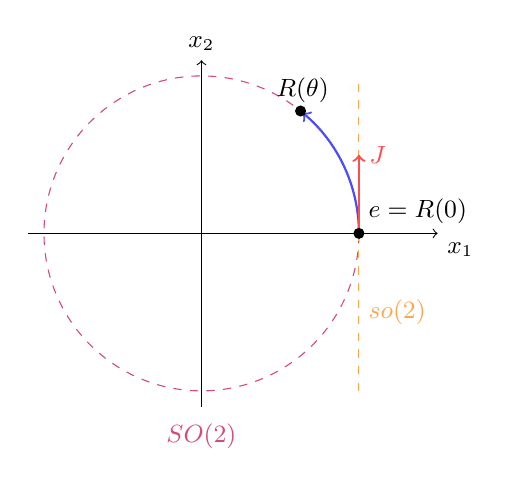
\begin{tikzpicture}[scale=1,every node/.style={font=\small}]
            \draw[->] (-2.2,0) -- (3,0) node[below right] {$x_1$};
            \draw[->] (0,-2.2) -- (0,2.2) node[above] {$x_2$};

            \draw[dashed, purple!70] (0,0) circle (2cm);
            \node[below, purple!70] at (0,-2.3) {$SO(2)$};

            \draw[->, thick, blue!70] (2,0) arc (0:50:2);
            \fill ({2*cos(51)},{2*sin(51)}) circle (2pt);
            \node[above] at ({2*cos(50)},{2*sin(50)}) {$R(\theta)$};

            \draw[dashed,orange!70] (2,-2) -- (2,2);
            \draw[->, red!70, thick] (2,0) -- +(0,1) node[right] {$J$};
            \node[right,orange!70] at (2,-1) {$\mathfrak{so}(2)$};

            \fill (2,0) circle (2pt) node[above right] {$e=R(0)$};
        \end{tikzpicture}
    \end{minipage}
\end{figure}

\textbf{Common Lie groups:}
\begin{itemize}
    \item $\mathbf{O(n)} = \{ R \in \mathbb{R}^{n \times n} \mid R^T R = I \}$: orthogonal group, preserves Euclidean lengths.
    \item $\mathbf{SO(n)} = \{ R \in O(n) \mid \det R = 1 \}$: special orthogonal group, proper rotations in $n$ dimensions.
    \item $\mathbf{U(n)} = \{ U \in \mathbb{C}^{n \times n} \mid U^\dagger U = I \}$: unitary group, preserves complex inner products.
    \item $\mathbf{SU(n)} = \{ U \in U(n) \mid \det U = 1 \}$: special unitary group, important for internal symmetries in particle physics.
          % \item $\mathbf{Sp(2n)} = \{ M \in \mathbb{R}^{2n \times 2n} \mid M^T \Omega M = \Omega \}$: symplectic group, preserves a symplectic form $\Omega$ in classical and quantum mechanics.
\end{itemize}

\subsection{Representations}

A \textbf{representation} of a Lie group or Lie algebra provides a concrete realization of its abstract elements as linear operators acting on a vector space.
Mathematically, a representation of a Lie group \(G\) is a homomorphism, for example
\[
    D : G \to \mathrm{GL}(V),
\]
where \(V\) is the vector space on which our representation is acting and \(\mathrm{GL}(V)\) denotes the group of invertible linear transformations on \(V\).
This means that the group law is preserved:
\[
    D(g_1 g_2) = D(g_1) D(g_2), \qquad \forall g_1,g_2 \in G.
\]
At the infinitesimal level, a representation of the associated Lie algebra \(\mathfrak{g}\) assigns to each generator \(T_a\) a linear operator \(D(T_a)\) such that
\[
    [D(T_a), D(T_b)] = i f_{ab}{}^{c} D(T_c),
\]
mirroring the structure constants \(f_{ab}{}^{c}\) of the algebra.

Representations are fundamental both in mathematics and in physics.
Mathematically, they allow us to study abstract symmetry groups through their action on vector spaces, revealing their structure via matrices or operators.
Physically, they describe how different objects transform under a given symmetry:
scalars correspond to the trivial (one-dimensional) representation,
vectors to the fundamental representation, and spinors or tensors to higher-dimensional or mixed representations.

Of particular importance are the \textbf{irreducible representations}, which cannot be decomposed into smaller invariant subspaces.
These play the role of the "elementary building blocks" of a group—just as elementary particles of definite spin are the basic excitations transforming irreducibly under spacetime symmetries.

Different Lie groups admit representations of various \textbf{dimensions}, depending on how the group acts on the underlying vector space.
For example, the group $SO(2)$ can be represented by $2\times 2$ rotation matrices acting on vectors in the plane, but also by complex phase factors $e^{i n \theta}$ acting on one-dimensional complex spaces, each labeled by an integer $n$.
In general, higher-dimensional representations describe systems that transform with more internal components---such as vectors, tensors, or spinors---while lower-dimensional ones correspond to simpler transformation laws.
The dimension of the representation thus reflects the number of independent degrees of freedom that transform under the symmetry.
